\documentclass[11pt,a4paper,titlepage]{article}
\usepackage[a4paper]{geometry}
\usepackage[utf8]{inputenc}
\usepackage[english]{babel}
\usepackage{lipsum}
\usepackage{eurosym}
\usepackage{rotating}

\usepackage{amsmath, amssymb, amsfonts, amsthm, mathtools}
% mathtools for: Aboxed (put box on last equation in align environment)
\usepackage{microtype} %improves the spacing between words and letters

\usepackage{lipsum}
\usepackage{threeparttable}
\usepackage{tabularx}
\usepackage{multirow}
\usepackage{booktabs}
\newcommand{\tabitem}{~~\llap{\textbullet}~~}
\usepackage{graphicx}
\graphicspath{ {./figures/} {./eps/}}
\usepackage{epsfig}
\usepackage{epstopdf}
\usepackage{verbatim}
\usepackage{textcomp}
\usepackage{tikz}
\usetikzlibrary{shapes,arrows}

%%%%%%%%%%%%%%%%%%%%%%%%%%%%%%%%%%%%%%%%%%%%%%%%%%
%% COLOR DEFINITIONS
%%%%%%%%%%%%%%%%%%%%%%%%%%%%%%%%%%%%%%%%%%%%%%%%%%
 % Enabling mixing colors and color's call by 'svgnames'
%%%%%%%%%%%%%%%%%%%%%%%%%%%%%%%%%%%%%%%%%%%%%%%%%%
\definecolor{MyColor1}{HTML}{CC0000} %mix personal color
\newcommand{\textb}{\color{Black} \usefont{OT1}{lmss}{m}{n}}
\newcommand{\blue}{\color{MyColor1} \usefont{OT1}{lmss}{m}{n}}
\newcommand{\blueb}{\color{MyColor1} \usefont{OT1}{lmss}{b}{n}}
\newcommand{\red}{\color{LightCoral} \usefont{OT1}{lmss}{m}{n}}
\newcommand{\green}{\color{Turquoise} \usefont{OT1}{lmss}{m}{n}}
%%%%%%%%%%%%%%%%%%%%%%%%%%%%%%%%%%%%%%%%%%%%%%%%%%

%%%%%%%%%%%%%%%%%%%%%%%%%%%%%%%%%%%%%%%%%%%%%%%%%%
%% Scala coloring settings
%%%%%%%%%%%%%%%%%%%%%%%%%%%%%%%%%%%%%%%%%%%%%%%%%%
% "define" Scala
\usepackage{listings}
\usepackage{xcolor}
\lstset{escapeinside={<@}{@>}}

\definecolor{dkgreen}{rgb}{0,0.6,0}
\definecolor{gray}{rgb}{0.5,0.5,0.5}
\definecolor{mauve}{rgb}{0.58,0,0.82}
\definecolor{cri1}{HTML}{2D85FF}
\definecolor{cri2}{HTML}{FF006E}
\definecolor{cri3}{HTML}{0008FF}
\definecolor{cri4}{HTML}{00A9FF}
\definecolor{cri5}{HTML}{55CF7D}
\definecolor{cri6}{HTML}{FFAF1C}

\lstdefinestyle{myScalastyle}{
  frame=tb,
  language=scala,
  aboveskip=3mm,
  belowskip=3mm,
  showstringspaces=false,
  columns=flexible,
  basicstyle={\small\ttfamily},
  numbers=none,
  numberstyle=\tiny\color{gray},
  keywordstyle=\color{blue},
  commentstyle=\color{dkgreen},
  stringstyle=\color{mauve},
  frame=single,
  breaklines=true,
  breakatwhitespace=true,
  tabsize=3,
}

\lstdefinestyle{myBashstyle}{
  frame=tb,
  language=bash,
  aboveskip=3mm,
  belowskip=3mm,
  showstringspaces=false,
  columns=flexible,
  basicstyle={\small\ttfamily},
  numbers=none,
  numberstyle=\tiny\color{gray},
  keywordstyle=\color{cri2},
  commentstyle=\color{cri1},
  stringstyle=\color{cri6},
  % <@\textcolor{cri5}{'Ziggy is running the Recommender...'}@>
  % <@\textcolor{cri5}{'Adding dataset to Hadoop...'}@>
  % <@\textcolor{cri5}{'Creating directory...'}@>
  % <@\textcolor{cri5}{'Adding user_artist_data.txt...'}@>
  % <@\textcolor{cri5}{'Adding artist_data.txt...'}@>
  % <@\textcolor{cri5}{'Adding artist_alias.txt...'}@>
  frame=single,
  breaklines=true,
  breakatwhitespace=true,
  tabsize=3,
}

% \lstset{basicstyle=\ttfamily,
%   frame=tb,
%   aboveskip=3mm,
%   belowskip=3mm,
%   showstringspaces=false,
%   commentstyle=\color{cri1},
%   keywordstyle=\color{cri2},
% }

% \lstdefinelanguage{JavaScript}{
%   keywords={typeof, new, true, false, catch, function, return, null, catch, switch, var, if, in, while, do, else, case, break},
%   keywordstyle=\color{cri3}\bfseries,
%   ndkeywords={class, export, boolean, throw, implements, import, this},
%   ndkeywordstyle=\color{cri4}\bfseries,
%   identifierstyle=\color{black},
%   sensitive=false,
%   comment=[l]{//},
%   morecomment=[s]{/*}{*/},
%   commentstyle=\color{cri5}\ttfamily,
%   stringstyle=\color{cri6}\ttfamily,
%   morestring=[b]',
%   morestring=[b]"
% }
%
% \lstdefinestyle{myJavastyle}{
%    frame=tb,
%    aboveskip=3mm,
%    belowskip=3mm,
%    language=JavaScript,
%    backgroundcolor=\color{lightgray},
%    extendedchars=true,
%    basicstyle=\footnotesize\ttfamily,
%    showstringspaces=false,
%    showspaces=false,
%    numbers=left,
%    numberstyle=\footnotesize,
%    numbersep=9pt,
%    tabsize=2,
%    breaklines=true,
%    showtabs=false,
%    captionpos=b
% }
%%%%%%%%%%%%%%%%%%%%%%%%%%%%%%%%%%%%%%%%%%%%%%%%%%
%% FONTS AND COLORS
%%%%%%%%%%%%%%%%%%%%%%%%%%%%%%%%%%%%%%%%%%%%%%%%%%
%		SECTIONS
%%%%%%%%%%%%%%%%%%%%%%%%%%%%%%%%%%%%%%%%%%%%%%%%%%
\usepackage{titlesec}
\usepackage{sectsty}
%%%%%%%%%%%%%%%%%%%%%%%%
%set section/subsections HEADINGS font and color
\sectionfont{\color{MyColor1}}  % sets colour of sections
\subsectionfont{\color{MyColor1}}  % sets colour of sections

%set section enumerator to arabic number (see footnotes markings alternatives)
\renewcommand\thesection{\arabic{section}.} %define sections numbering
\renewcommand\thesubsection{\thesection\arabic{subsection}} %subsec.num.

%define new section style
\newcommand{\mysection}{
\titleformat{\section} [runin] {\usefont{OT1}{lmss}{b}{n}\color{MyColor1}}
{\thesection} {3pt} {} }

%%%%%%%%%%%%%%%%%%%%%%%%%%%%%%%%%%%%%%%%%%%%%%%%%%
%		CAPTIONS
%%%%%%%%%%%%%%%%%%%%%%%%%%%%%%%%%%%%%%%%%%%%%%%%%%
\usepackage{caption}
\usepackage{subcaption}
%%%%%%%%%%%%%%%%%%%%%%%%
\captionsetup[figure]{labelfont={color=MyColor1}}

%%%%%%%%%%%%%%%%%%%%%%%%%%%%%%%%%%%%%%%%%%%%%%%%%%
%		!!!EQUATION (ARRAY) --> USING ALIGN INSTEAD
%%%%%%%%%%%%%%%%%%%%%%%%%%%%%%%%%%%%%%%%%%%%%%%%%%
%using amsmath package to redefine eq. numeration (1.1, 1.2, ...)
%%%%%%%%%%%%%%%%%%%%%%%%
\renewcommand{\theequation}{\thesection\arabic{equation}}

%set box background to grey in align environment
\usepackage{etoolbox}% http://ctan.org/pkg/etoolbox
\makeatletter
\patchcmd{\@Aboxed}{\boxed{#1#2}}{\colorbox{black!15}{$#1#2$}}{}{}%
\patchcmd{\@boxed}{\boxed{#1#2}}{\colorbox{black!15}{$#1#2$}}{}{}%
\makeatother
%%%%%%%%%%%%%%%%%%%%%%%%%%%%%%%%%%%%%%%%%%%%%%%%%%

\newcommand{\DP}[1]{\textcolor{blue}{\textbf{(DP says: #1)}}}
\newcommand{\cri}[1]{\textcolor{green}{\textbf{(Cri says: #1)}}}

\makeatletter
\let\reftagform@=\tagform@
\def\tagform@#1{\maketag@@@{(\ignorespaces\textcolor{red}{#1}\unskip\@@italiccorr)}}
\renewcommand{\eqref}[1]{\textup{\reftagform@{\ref{#1}}}}
\makeatother
\usepackage[hidelinks]{hyperref}

%% LISTS CONFIGURATION %%
\usepackage{enumitem}
\setlist[enumerate,1]{start=0}
\renewcommand{\labelenumii}{\theenumii}
\renewcommand{\theenumii}{\theenumi.\arabic{enumii}.}

\usepackage[acronym]{glossaries}
\newacronym{pmu}{PMU}{Power Management Unit}
\newacronym{pcb}{PCB}{Printed Circuit Board}
\newacronym{ic}{IC}{Integrated Circuit}
\newacronym{emc}{EMC}{Electromagnetic compatibility}
\newacronym{smd}{SMD}{Surface Mounted Device}

%%%%%%%%%%%%%%%%%%%%%%%%%%%%%%%%%%%%%%%%%%%%%%%%%%
%% PREPARE TITLE
%%%%%%%%%%%%%%%%%%%%%%%%%%%%%%%%%%%%%%%%%%%%%%%%%%
\title{\blue SIBD final project}
\author{Davide Peron\\ Cristina Gava}
\date{\today}
%%%%%%%%%%%%%%%%%%%%%%%%%%%%%%%%%%%%%%%%%%%%%%%%%%

\begin{document}
\maketitle
\section{Solution's implementation}
The first step to do was the execution of the Recommender in IntelliJ, using the Spark and Scala packets. To do it we firstly cleaned the dataset and took a subset of it in order to have a faster execution of the code. The dataset had to be cleaned from spurious characters which where present in artists' names and were not recognized as standard ASCII, and the code used for that is in the file \textit{$filter\_artist\_data.py$} and is shown here for completeness.

\begin{lstlisting}[style=myScalastyle]
inputfile=open("artist_data.txt", "r")
outputfile = open("artist_data_filtered.txt", "w")
i = 0

for line in inputfile:
    line_array = line.split("\t")
    i += 1
    if(len(line_array) == 2):
        outputfile.write(line)
\end{lstlisting}

After that we took a subset of artist data, which now is 184 Bytes long: we are aware that this dimension corresponds only to a few lines from the dataset, but  we did so in order to execute the recommender in a little amount of time, given the power of our laptops. Using decentralized web services like AWS we would have been able to run the entire dataset, however the results of the code can be appreciated also with our small subset.

The next step was to modify the Recommender file code to make it execute on our machine: as it can be seen from the code below, first of all we imported the $Source$ library in order to deploy the args[] option and make the userID readable from command line. After that we declared the url for the hadoop server and port and made the code able to read the text files containing the dataset. Finally we added some \textit{println} instructions to see the evolution of each subsection of the code.

\begin{lstlisting}[style=myScalastyle]
import scala.io.Source

object RunRecommender {

  def main(args: Array[String]): Unit = {

    Logger.getLogger("org").setLevel(Level.OFF)
    Logger.getLogger("akka").setLevel(Level.OFF)

        val userID = args(0).toInt
    val spark = SparkSession.builder().master("local").getOrCreate()
    // Optional, but may help avoid errors due to long lineage
    // spark.sparkContext.setCheckpointDir("hdfs://localhost:54310/tmp/")

    //val base = "hdfs://localhost:54310/user/ds/"
        val base = "hdfs://hadoop:9000/user/ds/"
    val rawUserArtistData = spark.read.textFile(base + "user_artist_data.txt")
    val rawArtistData = spark.read.textFile(base + "artist_data_filtered.txt")
    val rawArtistAlias = spark.read.textFile(base + "artist_alias.txt")

    val runRecommender = new RunRecommender(spark)
    println("Preparation")
    runRecommender.preparation(rawUserArtistData, rawArtistData, rawArtistAlias)
    println("Model")
    runRecommender.model(rawUserArtistData, rawArtistData, rawArtistAlias, userID)
    println("Evaluation")
    runRecommender.evaluate(rawUserArtistData, rawArtistAlias)
    println("Recommendation")
    runRecommender.recommend(rawUserArtistData, rawArtistData, rawArtistAlias)
  }
\end{lstlisting}
\section{SBT dependencies}
The dependencies for the Recommender have been managed through the $build.sbt$ file, here shown below.

\begin{lstlisting}[style=myScalastyle]
name := "RecommenderSBT"

version := "0.1"

scalaVersion := "2.11.12"

val sparkVer = "2.1.0"

libraryDependencies ++= Seq(
  "org.apache.spark" %% "spark-core" % sparkVer,
  "org.apache.spark" %% "spark-sql" % sparkVer,
  "org.apache.spark" %% "spark-mllib" % sparkVer,
  "com.github.fommil.netlib" % "all" % "1.1.2" pomOnly()
)
\end{lstlisting}
\section{HDFS File System using Hadoop}
To correctly run the recommender we used the HDFS file system offered by Apache Hadoop.
Here we uploaded the dataset we have to analyse and we wrote in the recommender code where to take the data from with the syntax \textit{hdfs://host\_name:port/path/of/dataset}.

The whole code then has been executed in the IntelliJ IDE and the recommender gave a few suggestions for the selected user.

\section{Docker containers configuration}
For the implementation in Docker we created a $Docker ~Compose$ file in which we listed the two services for Hadoop and Spark. The code contained in the file is listed here:

\begin{lstlisting}[style=myBashstyle]
version: '2'
services:
  spark:
    image: "p7hb/docker-spark:2.1.0"
    container_name: spark
    volumes:
      - ./shared:/shared
    ports:
      - 4040:4040
      - 8080:8080
      - 8081:8081
    command: bash -c "/shared/spark_setup.sh"
  hadoop:
    image: "sequenceiq/hadoop-docker:2.7.1"
    container_name: hadoop
    volumes:
      - ./shared:/shared
    ports:
      - 9000:9000
    command: bash -c "/etc/bootstrap.sh -bash && /shared/db_setup.sh"
\end{lstlisting}

As it can be seen from the code, we first declared the Spark service and the ports through which make the container available.

The first thing that Docker Compose does, if not already done, is to pull the images of both the containers used in the services.
We also created a directory which is in common between the two containers, in order to upload the dataset only in one place and offer an environment in which the containers could share files without problems. The same settings have been modelled for Hadoop.

An important part in the yml file is the definition of the command files $spark\_setup.sh$ and $db\_setup.sh$. During the first attempts with the code we incurred in some problems regarding the order of execution of the services: we noticed that sometimes the program was crashing due to the fact that Spark required the dataset before Hadoop was able to fully set the connection to it. So we wrote:
\begin{itemize}
\item \textbf{spark\_setup.sh}
\end{itemize}
\begin{lstlisting}[style=myBashstyle]
/bin/echo <@\textcolor{cri5}{'Welcome in Ziggy, the new generation of Recommender!!'}@>
/bin/echo '

#I keep Spark sleeping until Hadoop is not ready
while [ ! -e /shared/ready.txt ]
do
    sleep 1
done

rm -rf /shared/ready.txt

#then I start the Recommender

/bin/echo <@\textcolor{cri5}{'Ziggy is running the Recommender...'}@>
spark-submit --class com.cloudera.datascience.recommender.RunRecommender /shared/recommender_2.11-0.1.jar 2093760
\end{lstlisting}
and
\begin{itemize}
\item \textbf{db\_setup.sh}
\end{itemize}
\begin{lstlisting}[style=myBashstyle]
/bin/echo <@\textcolor{cri5}{'Adding dataset to Hadoop...'}@>

#Adding Hadoop to PATH
PATH="$PATH:/usr/local/hadoop/bin"
hdfs dfsadmin -safemode leave

#Adding dataset to Hadoop checking that it doesn't exists yet

hadoop fs -test -e /user/ds
if [ $? != 0 ]
then
    /bin/echo <@\textcolor{cri5}{reating directory...'}@>
    hadoop fs -mkdir /user/ds
fi

hadoop fs -test -e /user/ds/user_artist_data.txt
if [ $? != 0 ]
then
    /bin/echo <@\textcolor{cri5}'<{dding user\_artist\_data.txt...'}@>
    hadoop fs -put /shared/user_artist_data.txt /user/ds/user_artist_data.txt
fi

hadoop fs -test -e /user/ds/artist_data_filtered.txt
if [ $? != 0 ]
then
    /bin/echo <@\textcolor{cri5}{'Adding artist\_data.txt...'}@>
    hadoop fs -put /shared/artist_data_filtered.txt /user/ds/artist_data_filtered.txt
fi

hadoop fs -test -e /user/ds/artist_alias.txt
if [ $? != 0 ]
then
    /bin/echo <@\textcolor{cri5}{'Adding artist\_alias.txt...'}@>
    hadoop fs -put /shared/artist_alias.txt /user/ds/artist_alias.txt
fi

echo "I'm ready" >> /shared/ready.txt
chmod 777 /shared/ready.txt

while true
do
    sleep 1
done
\end{lstlisting}
In the $spark\_setup$ we said to Spark to wait until Hadoop is ready (it will understand when this moment comes checking the existence of $ready.txt$ file in the shared directory), at the same time the file \textit{Docker Compose} starts the Hadoop service and the correspondent container. When the Hadoop container is ready, the file $db\_setup$ executes: the first thing it does is to check if the dataset is already added, if not so, it is uploaded. When every file is ready, Hadoop creates the file $ready.txt$ setting its user permission to 777 mode (everyone has full access to the file) so as to be possible for the Spark service to read it and delete it after.

After the file creation, Hadoop enters a sort of \textit{listening} mode, in which it waits for the Spark container to run the recommender, and finally produces an $end.txt$ file.
So, while Hadoop is waiting, Spark detects the existence of $ready.txt$, it deletes it and runs the recommender. Once the recommender finished its tasks, the Spark service produces the $end.txt$ file with, again, 777 permissions and stops.

At this point Hadoop detects the $end.txt$ file and stops too.

An example of execution is shown in \autoref{fig:execution1} and \autoref{fig:execution2}.

% \begin{figure}[ht]
%     \centering
%     \begin{subfigure}[b]{.45\textwidth}
%         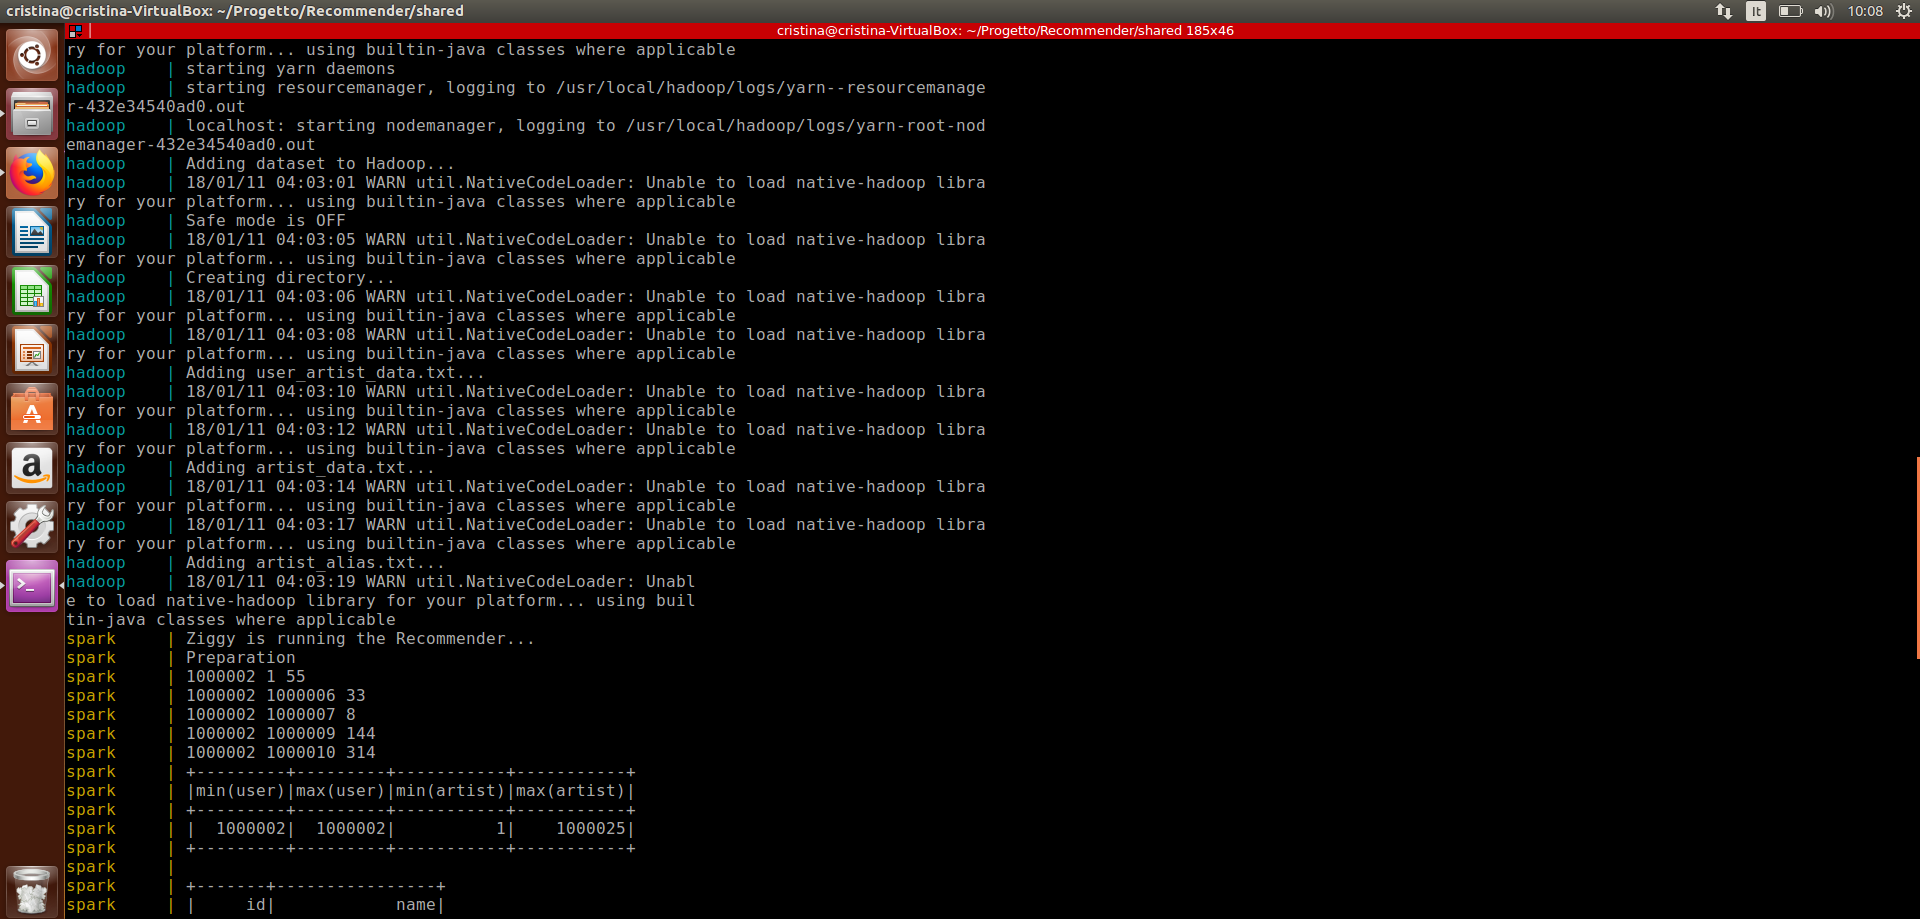
\includegraphics[width=\textwidth]{Screenshot(120).png}
%     \end{subfigure}
% 		\hspace{0.5cm}
% 		\begin{subfigure}[b]{.45\textwidth}
% 				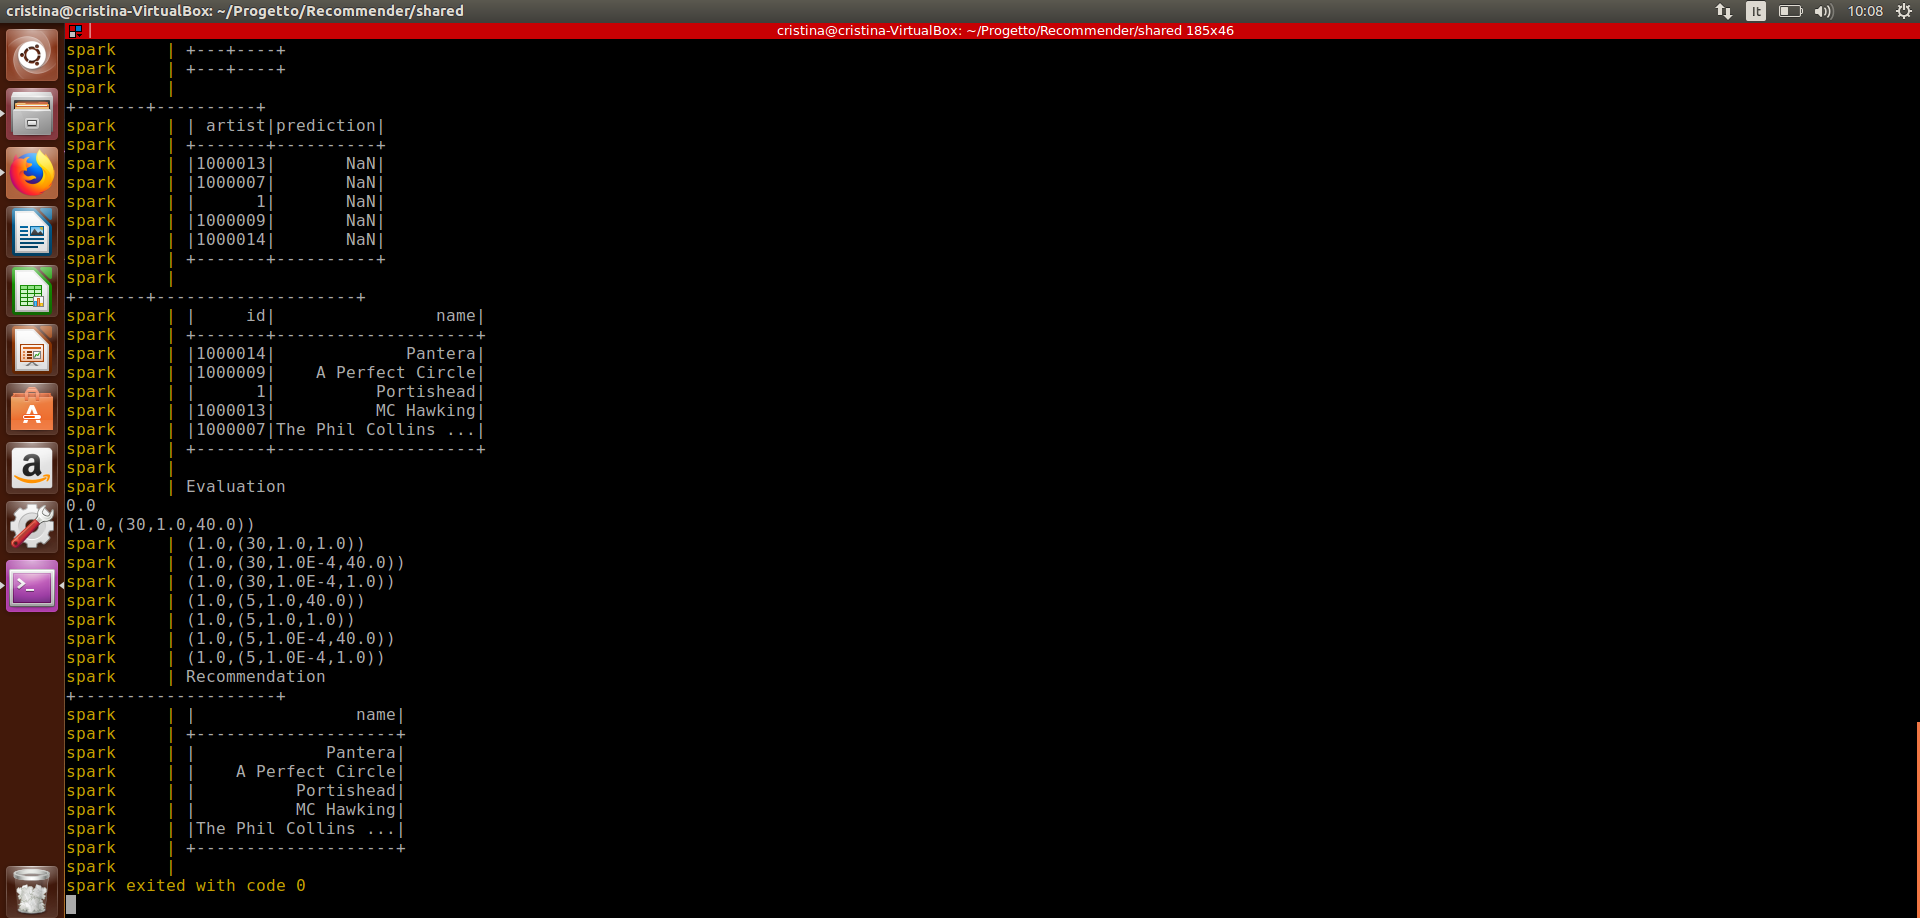
\includegraphics[width=\textwidth]{Screenshot(119).png}
% 		\end{subfigure}
% 		\caption{Example of execution of the Recommender using Docker Compose}
% 		\label{fig:execution}
% \end{figure}
\newpage
\begin{figure}[ht]
    \centering
        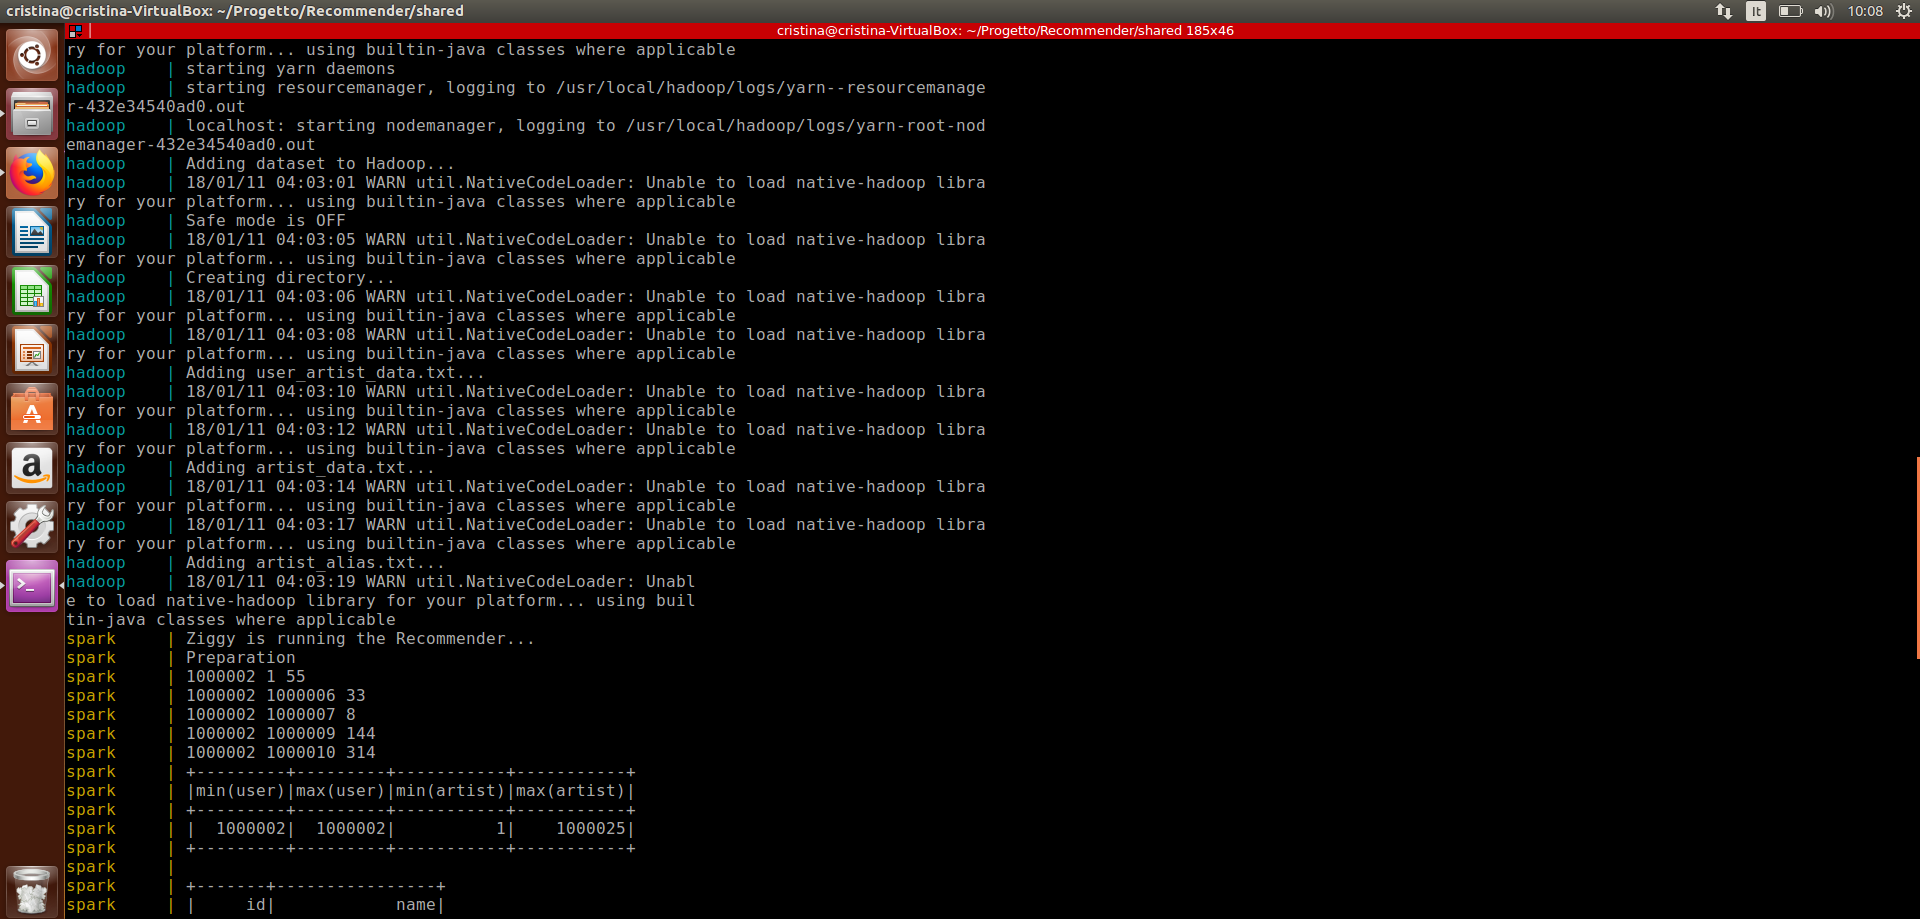
\includegraphics[width=0.8\textwidth]{Screenshot(120).png}
        \caption{Example of execution of the Recommender using Docker Compose}
        \label{fig:execution1}
\end{figure}
\begin{figure}[ht]
    \centering
				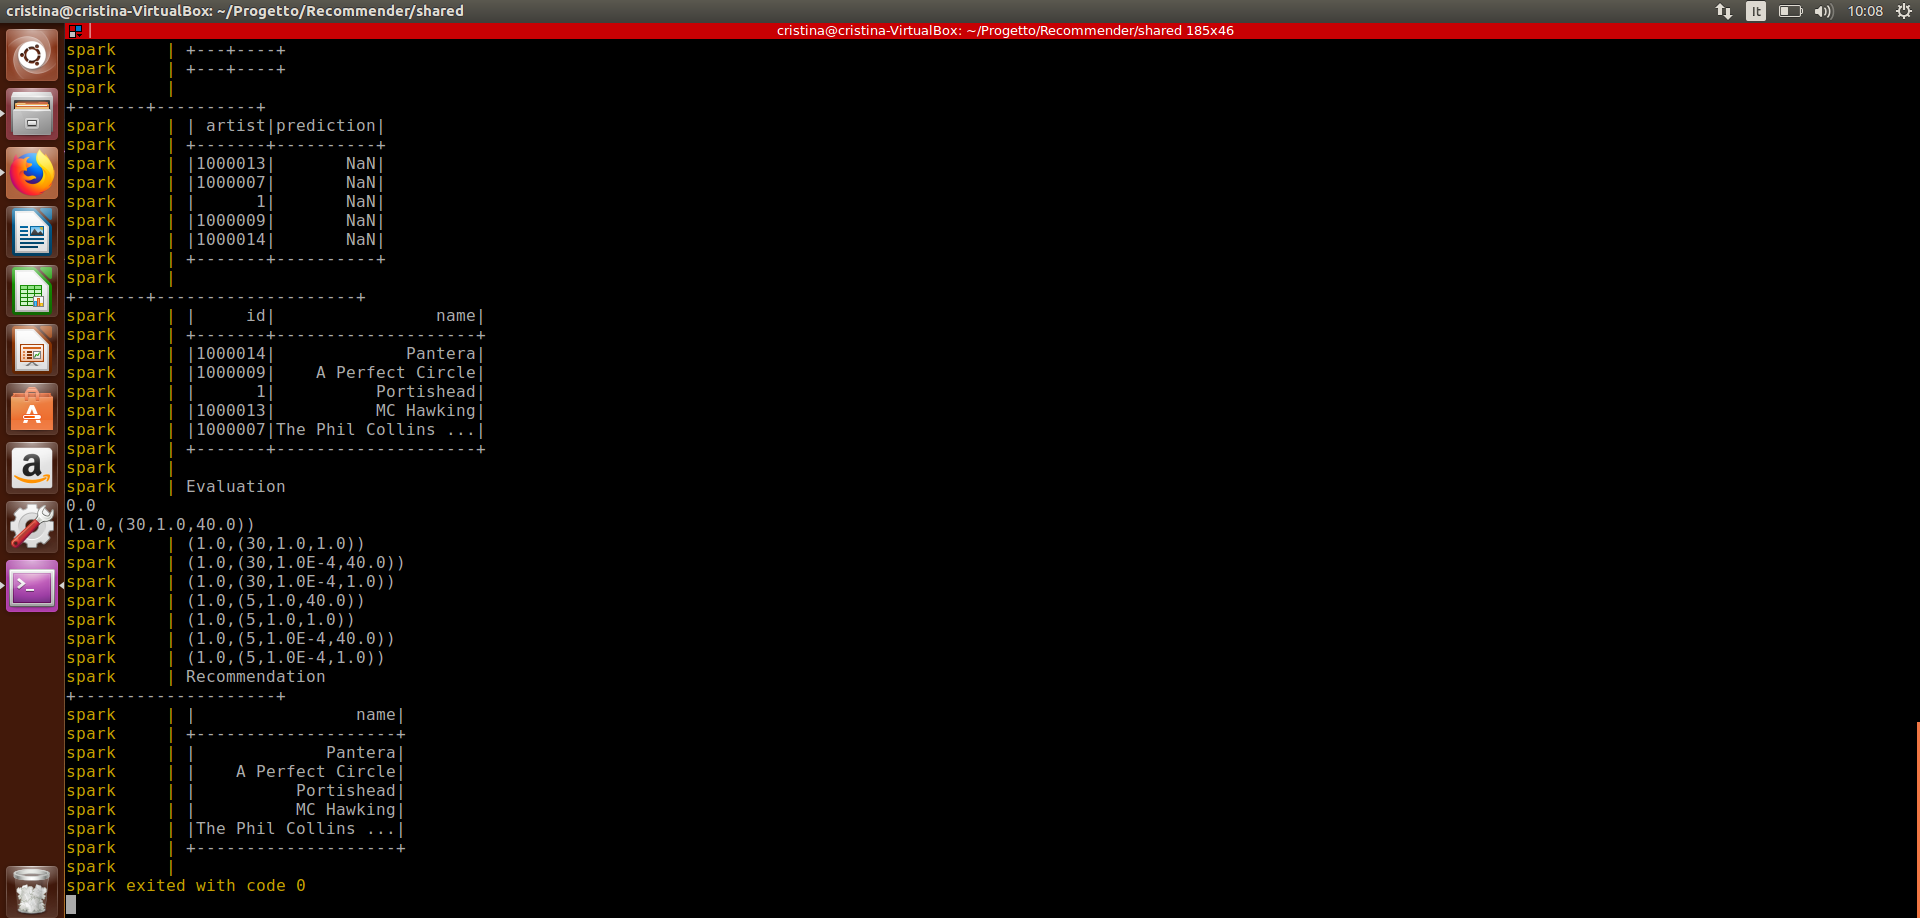
\includegraphics[width=0.8\textwidth]{Screenshot(119).png}
		      \caption{Example of execution of the Recommender using Docker Compose}
		        \label{fig:execution2}
\end{figure}
\end{document}
